\section{Schedule}

\begin{figure}[ht]
    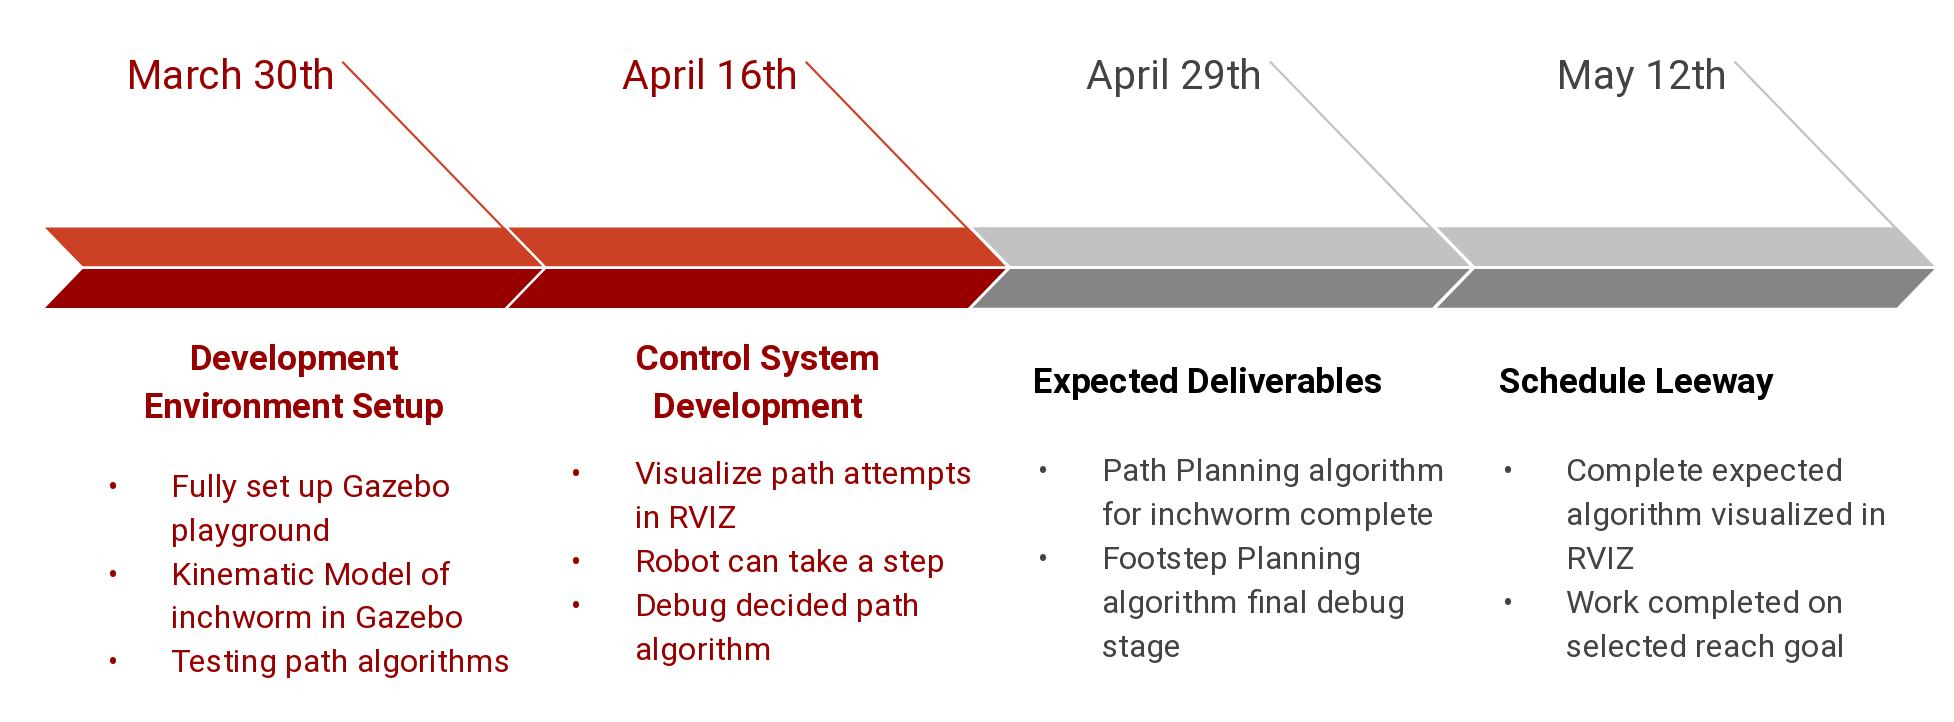
\includegraphics[width=\linewidth]{figures/Schedule.png}
    \caption{Proposed schedule for the project}
    \label{fig:Schedule}
\end{figure} 

The project has been split into three different sections: development environment setup, motion planning of the inchworm robot, and path planning of the inchworm. The development environment setup effort will be spearheaded by all 4 team members. After the environment is set up, two developers will be tasked with motion planning, while the other two will develop the path planning algorithms required. If all expected deliverables are completed, the team will re-evaluate the task division for reach goals. It is important to note that 2 weeks is dedicated to schedule leeway to deal with unexpected delays and/or development problems with previous tasks.